\documentclass[a4paper,12pt]{article}
\usepackage{xcolor}
\usepackage{amsmath,amsfonts,amssymb}
\usepackage{geometry}
\usepackage{fancyhdr}
\usepackage{graphicx}
\usepackage{titlesec}
\usepackage{tikz}
\usepackage{booktabs}
\usepackage{subcaption}
\usepackage{array}
\usetikzlibrary{shadows}
\usepackage{tcolorbox}
\usepackage{float}
\usepackage{lipsum}
\usepackage{mdframed}
\usepackage{pagecolor}
\usepackage{mathpazo}   % Palatino font (serif)
\usepackage{microtype}  % Better typography

% Page background color
\pagecolor{gray!10!white}

% Geometry settings
\geometry{margin=0.5in}
\pagestyle{fancy}
\fancyhf{}

% Fancy header and footer
\fancyhead[C]{\textbf{\color{blue!80}CS754 Assignment-1}}
% \fancyhead[R]{\color{blue!80}Saksham Rathi}
\fancyfoot[C]{\thepage}

% Custom Section Color and Format with Sans-serif font
\titleformat{\section}
{\sffamily\color{purple!90!black}\normalfont\Large\bfseries}
{\thesection}{1em}{}

% Custom subsection format
\titleformat{\subsection}
{\sffamily\color{cyan!80!black}\normalfont\large\bfseries}
{\thesubsection}{1em}{}

% Stylish Title with TikZ (Enhanced with gradient)
\newcommand{\cooltitle}[1]{%
  \begin{tikzpicture}
    \node[fill=blue!20,rounded corners=10pt,inner sep=12pt, drop shadow, top color=blue!50, bottom color=blue!30] (box)
    {\Huge \bfseries \color{black} #1};
  \end{tikzpicture}
}
\usepackage{float} % Add this package

\newenvironment{solution}[2][]{%
    \begin{mdframed}[linecolor=blue!70!black, linewidth=2pt, roundcorner=10pt, backgroundcolor=yellow!10!white, skipabove=12pt, skipbelow=12pt]%
        \textbf{\large #2}
        \par\noindent\rule{\textwidth}{0.4pt}
}{
    \end{mdframed}
}

% Document title
\title{\cooltitle{CS754 Assignment-3}}
\author{{\bf Saksham Rathi, Ekansh Ravi Shankar, Kshitij Vaidya}}
\date{}

\begin{document}
\maketitle
\textbf{Declaration:} The work submitted is our own, and
we have adhered to the principles of academic honesty while completing and submitting this work. We have not referred to any unauthorized sources, and we have not used generative AI tools for the work submitted here.

\section*{Question 3}

\begin{solution}{Solution}
  Here is the original cryoem image:
  \begin{figure}[H]
    \centering
    \begin{subfigure}[t]{0.32\textwidth}
        \centering
        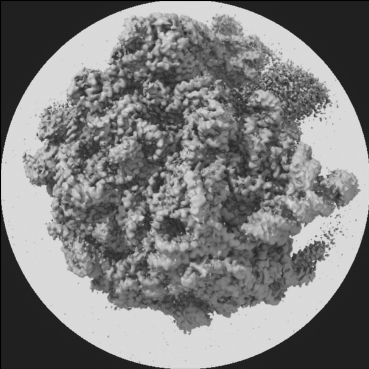
\includegraphics[width=\textwidth]{../images/cryoem.png}
        \caption*{$Original Image$}
    \end{subfigure}
    \label{fig:orig}
  \end{figure}

  Here are the steps followed:

  \begin{itemize}
    \item Generate random angles in the range [0, 360). (Number of angles decided by $N$.)
    \item Find the radon projections of the original image along these angles.
    \item Build the similarity matrix (using cosine similarity).
    \item Apply Laplacian eigenmaps to estimate projection angles.
    \item Normalize the angles, so that they belong to the range [0, 360).
    \item Reconstruct the image using inverse radon projections.
    \item Find the optimal rotation (to minimize RRMSE) (the number of angles tried is made to depend on the number of projections, for higher resolution, with the minimum number of angles tried to be 360).
  \end{itemize}

  \clearpage

  Here are the reconstructed images:



  \begin{figure}[H]
    \centering
    \begin{subfigure}[t]{0.32\textwidth}
        \centering
        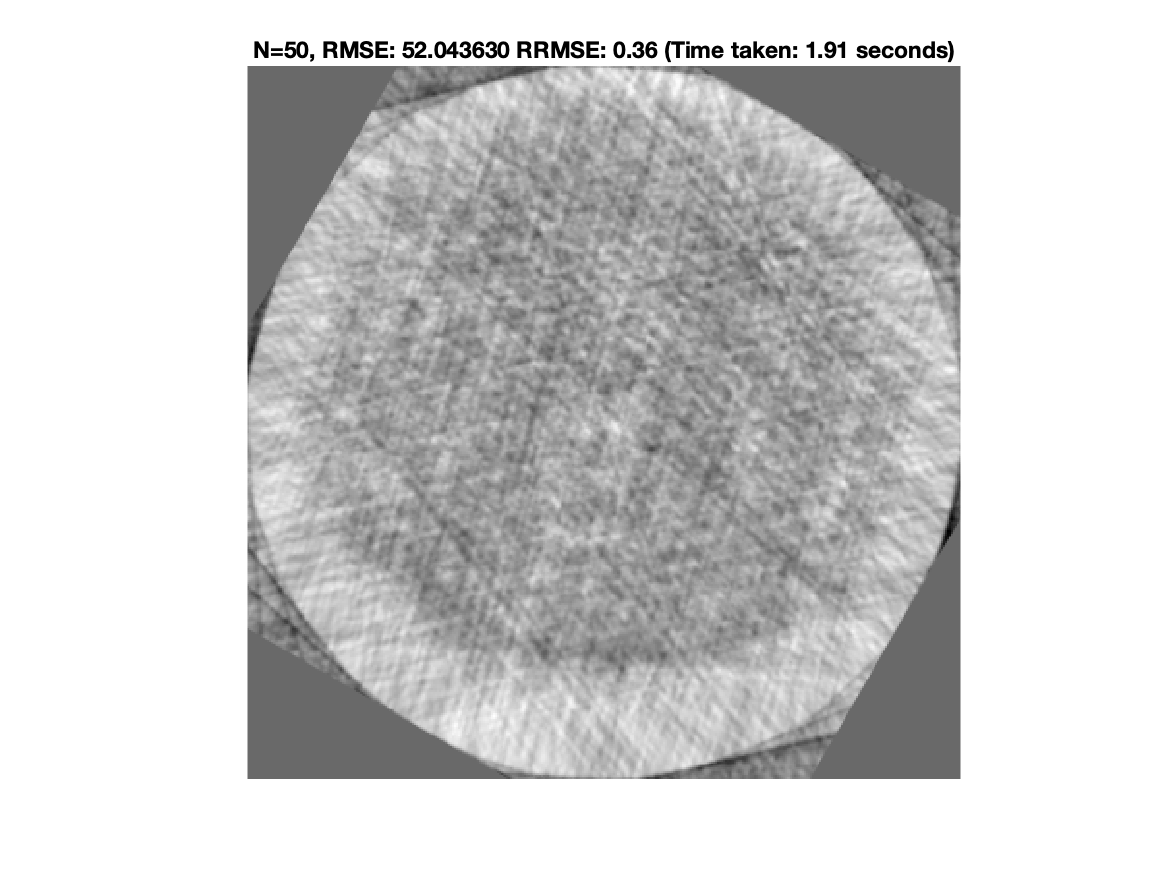
\includegraphics[width=\textwidth]{../images/reconstructed_N50.png}
        \caption*{$N = 50$}
    \end{subfigure}
    \begin{subfigure}[t]{0.32\textwidth}
        \centering
        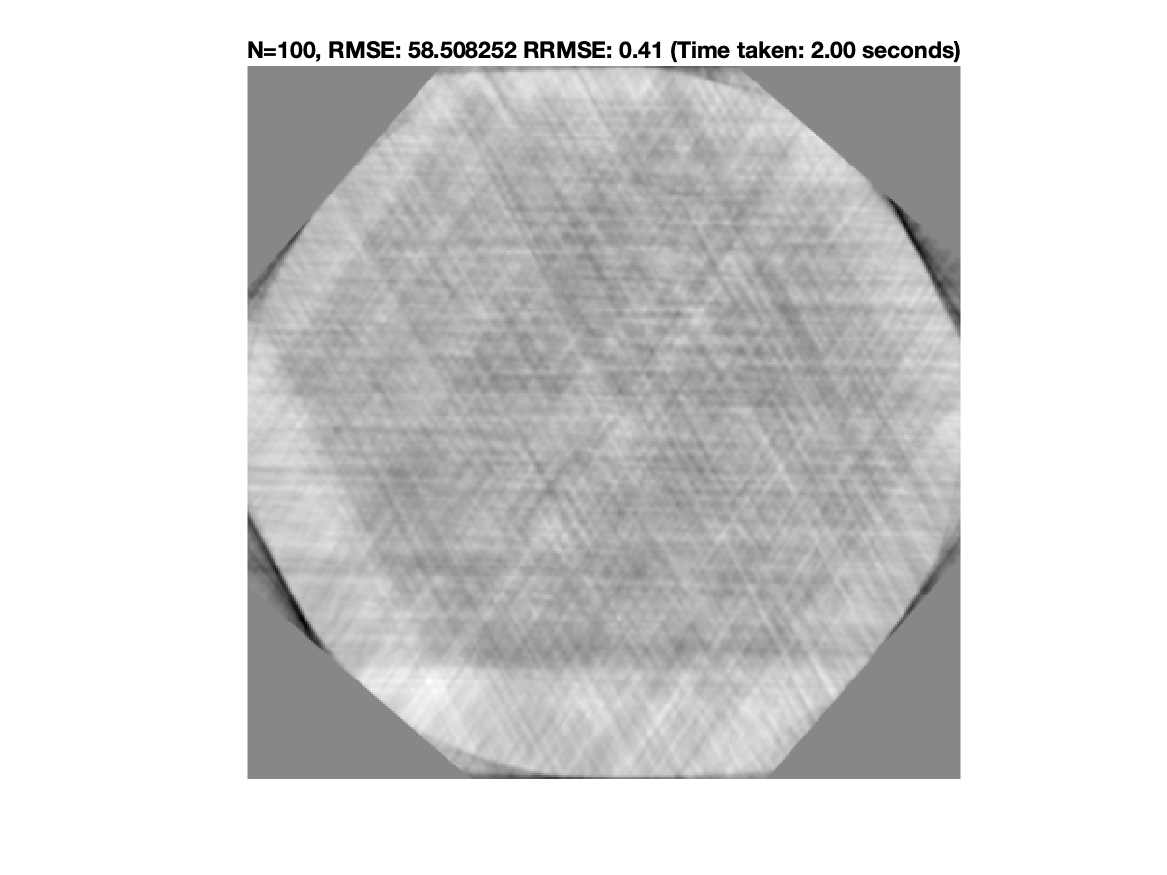
\includegraphics[width=\textwidth]{../images/reconstructed_N100.png}
        \caption*{$N = 100$}
    \end{subfigure}
    \begin{subfigure}[t]{0.32\textwidth}
        \centering
        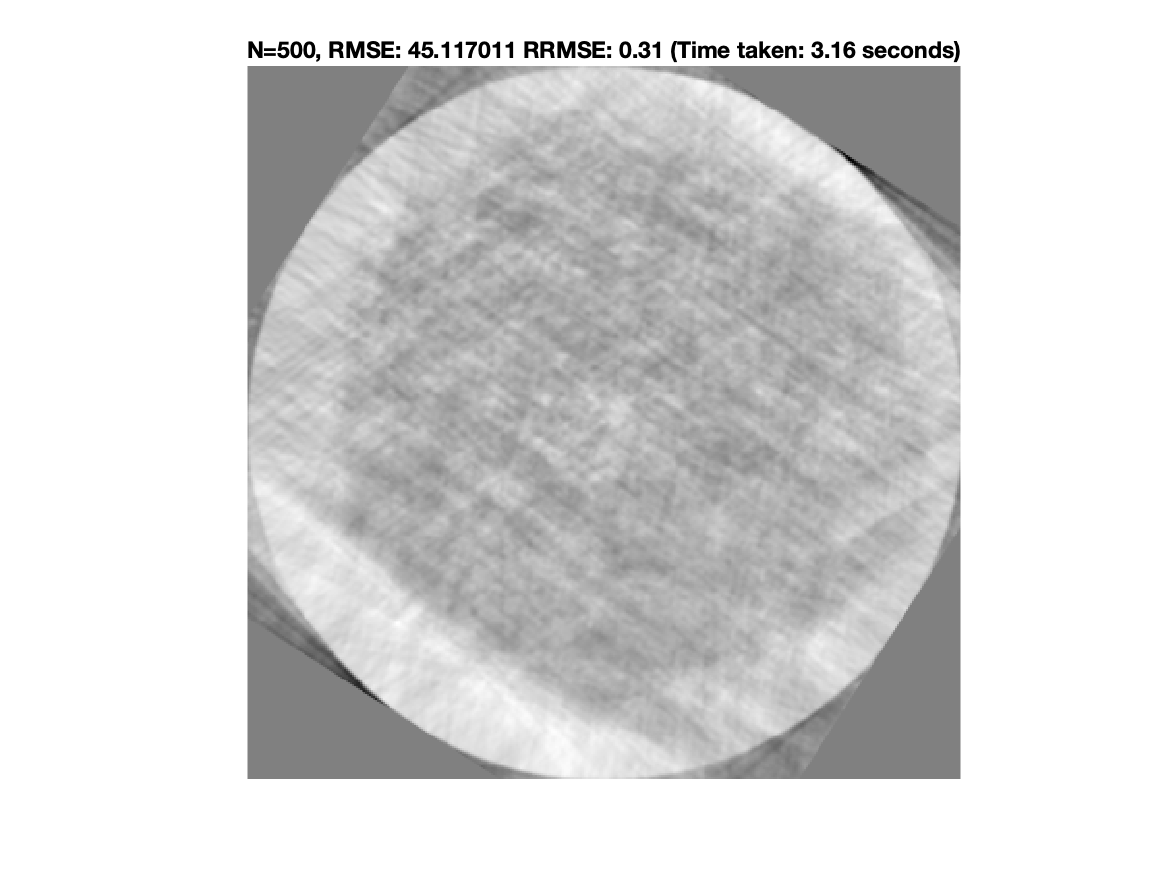
\includegraphics[width=\textwidth]{../images/reconstructed_N500.png}
        \caption*{$N = 500$}
    \end{subfigure}
    \label{fig:recons1}
  \end{figure}

  \begin{figure}[H]
    \centering
    \begin{subfigure}[t]{0.32\textwidth}
        \centering
        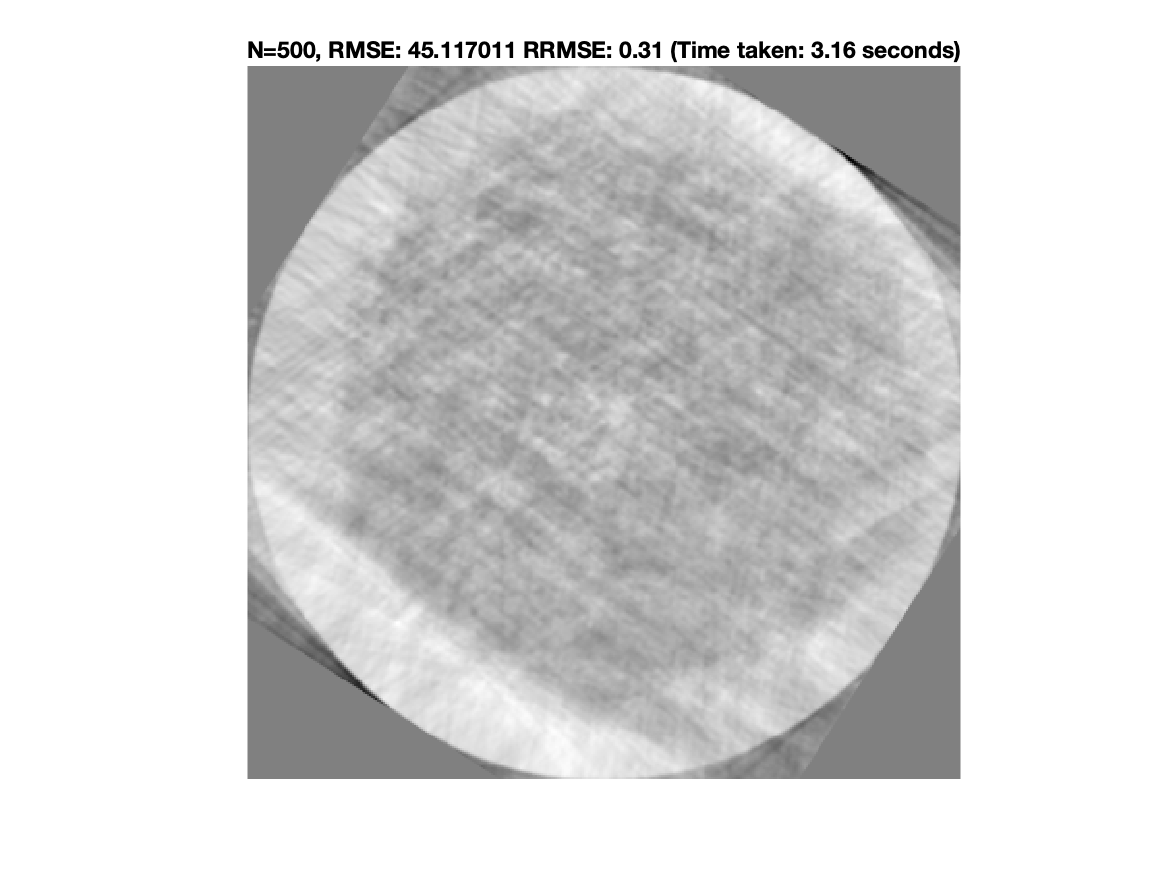
\includegraphics[width=\textwidth]{../images/reconstructed_N500.png}
        \caption*{$N = 500$}
    \end{subfigure}
    \begin{subfigure}[t]{0.32\textwidth}
        \centering
        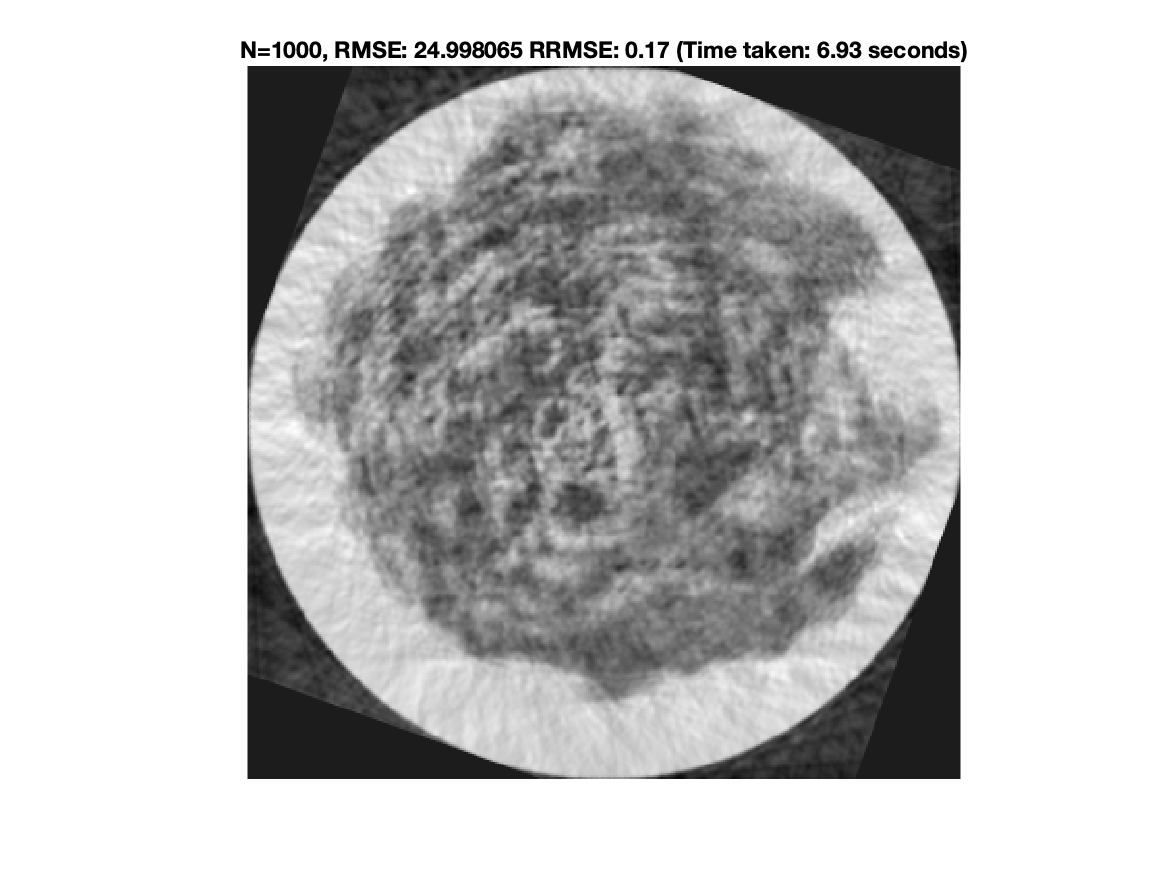
\includegraphics[width=\textwidth]{../images/reconstructed_N1000.png}
        \caption*{$N = 1000$}
    \end{subfigure}
    \begin{subfigure}[t]{0.32\textwidth}
        \centering
        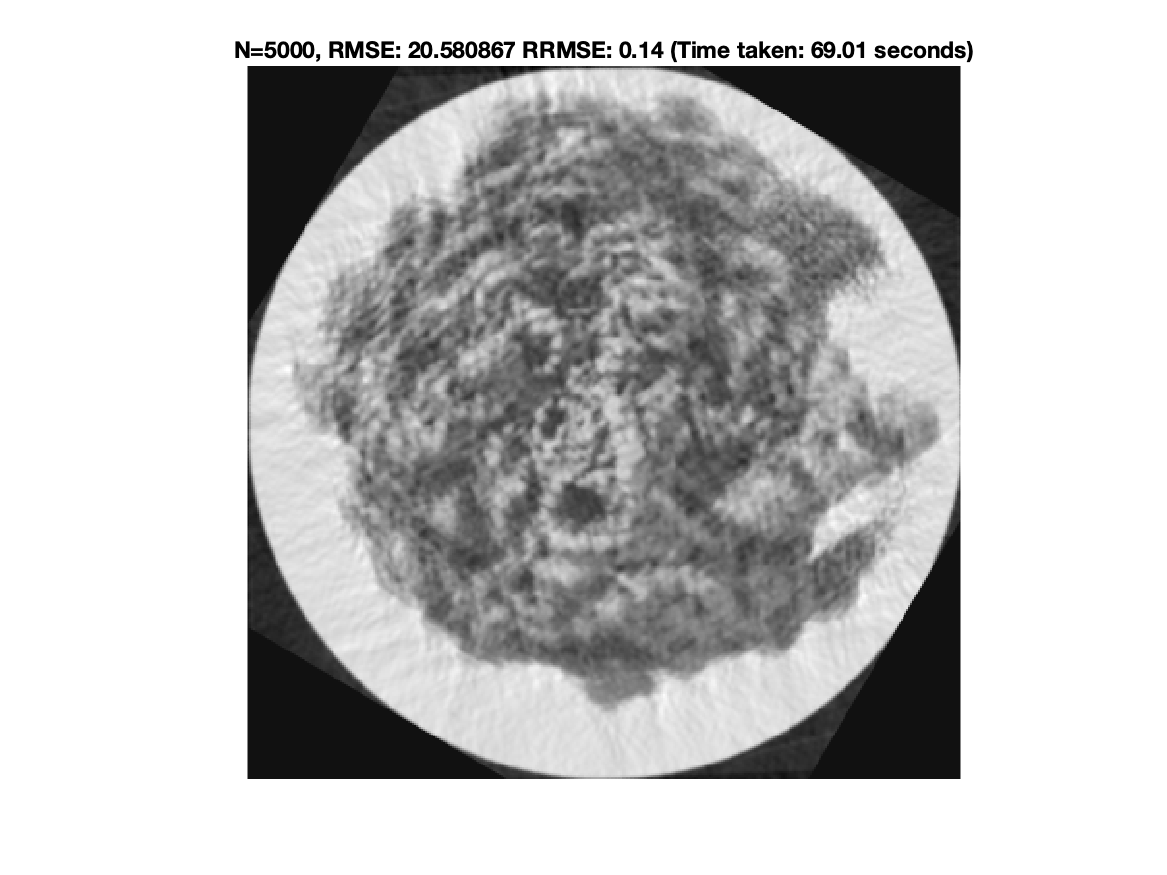
\includegraphics[width=\textwidth]{../images/reconstructed_N5000.png}
        \caption*{$N = 5000$}
    \end{subfigure}
    \label{fig:recons2}
  \end{figure}

  \begin{figure}[H]
    \centering
    \begin{subfigure}[t]{0.32\textwidth}
        \centering
        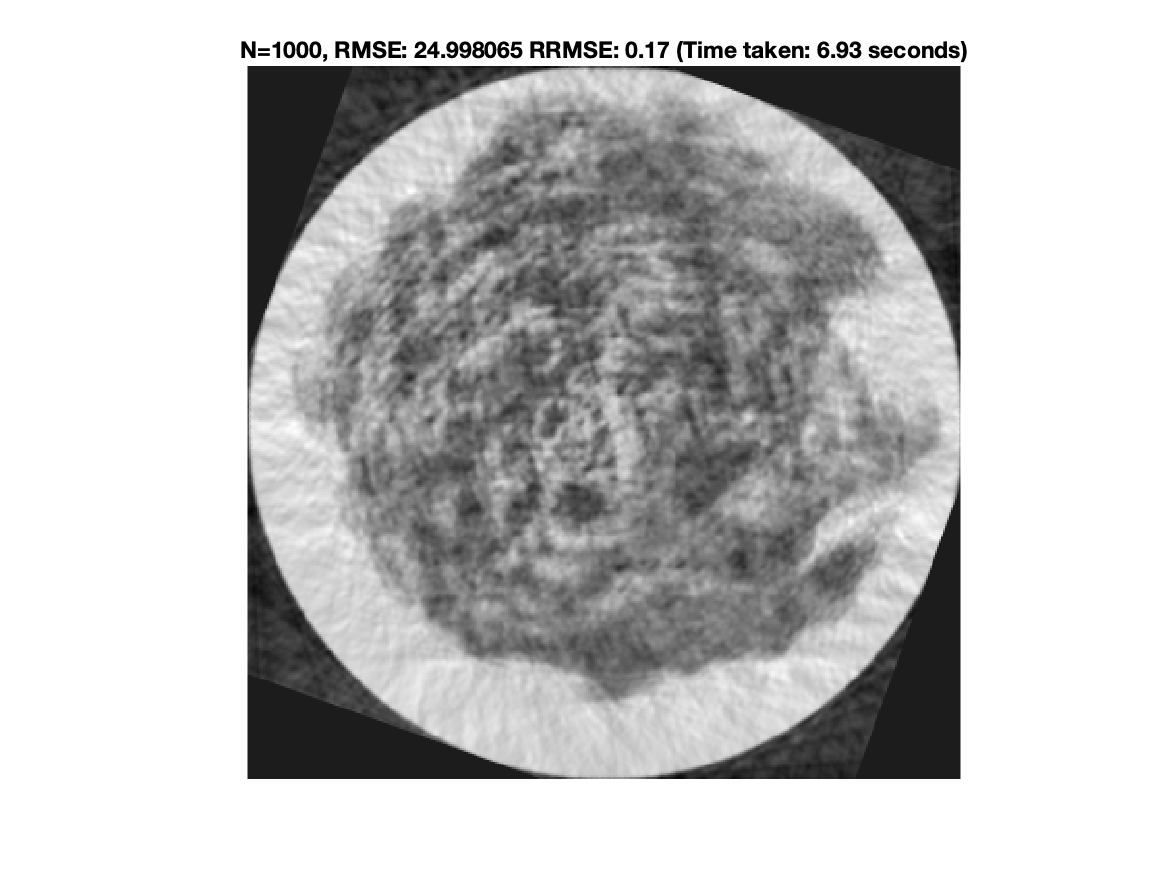
\includegraphics[width=\textwidth]{../images/reconstructed_N1000.png}
        \caption*{$N = 10000$}
    \end{subfigure}
    \caption*{Reconstructed image for different values of $N$}
    \label{fig:recons3}
  \end{figure}

  As we can see, the RRMSE (and RMSE) drops as N increases, which is expected, as we are getting data about more number of projections. Moreover, the image looks more similar to the original image. 

\end{solution}
\end{document}
